\documentclass[twoside]{book}

% Packages required by doxygen
\usepackage{fixltx2e}
\usepackage{calc}
\usepackage{doxygen}
\usepackage[export]{adjustbox} % also loads graphicx
\usepackage{graphicx}
\usepackage[utf8]{inputenc}
\usepackage{makeidx}
\usepackage{multicol}
\usepackage{multirow}
\PassOptionsToPackage{warn}{textcomp}
\usepackage{textcomp}
\usepackage[nointegrals]{wasysym}
\usepackage[table]{xcolor}

% Font selection
\usepackage[T1]{fontenc}
\usepackage[scaled=.90]{helvet}
\usepackage{courier}
\usepackage{amssymb}
\usepackage{sectsty}
\renewcommand{\familydefault}{\sfdefault}
\allsectionsfont{%
  \fontseries{bc}\selectfont%
  \color{darkgray}%
}
\renewcommand{\DoxyLabelFont}{%
  \fontseries{bc}\selectfont%
  \color{darkgray}%
}
\newcommand{\+}{\discretionary{\mbox{\scriptsize$\hookleftarrow$}}{}{}}

% Page & text layout
\usepackage{geometry}
\geometry{%
  a4paper,%
  top=2.5cm,%
  bottom=2.5cm,%
  left=2.5cm,%
  right=2.5cm%
}
\tolerance=750
\hfuzz=15pt
\hbadness=750
\setlength{\emergencystretch}{15pt}
\setlength{\parindent}{0cm}
\setlength{\parskip}{3ex plus 2ex minus 2ex}
\makeatletter
\renewcommand{\paragraph}{%
  \@startsection{paragraph}{4}{0ex}{-1.0ex}{1.0ex}{%
    \normalfont\normalsize\bfseries\SS@parafont%
  }%
}
\renewcommand{\subparagraph}{%
  \@startsection{subparagraph}{5}{0ex}{-1.0ex}{1.0ex}{%
    \normalfont\normalsize\bfseries\SS@subparafont%
  }%
}
\makeatother

% Headers & footers
\usepackage{fancyhdr}
\pagestyle{fancyplain}
\fancyhead[LE]{\fancyplain{}{\bfseries\thepage}}
\fancyhead[CE]{\fancyplain{}{}}
\fancyhead[RE]{\fancyplain{}{\bfseries\leftmark}}
\fancyhead[LO]{\fancyplain{}{\bfseries\rightmark}}
\fancyhead[CO]{\fancyplain{}{}}
\fancyhead[RO]{\fancyplain{}{\bfseries\thepage}}
\fancyfoot[LE]{\fancyplain{}{}}
\fancyfoot[CE]{\fancyplain{}{}}
\fancyfoot[RE]{\fancyplain{}{\bfseries\scriptsize Generated by Doxygen }}
\fancyfoot[LO]{\fancyplain{}{\bfseries\scriptsize Generated by Doxygen }}
\fancyfoot[CO]{\fancyplain{}{}}
\fancyfoot[RO]{\fancyplain{}{}}
\renewcommand{\footrulewidth}{0.4pt}
\renewcommand{\chaptermark}[1]{%
  \markboth{#1}{}%
}
\renewcommand{\sectionmark}[1]{%
  \markright{\thesection\ #1}%
}

% Indices & bibliography
\usepackage{natbib}
\usepackage[titles]{tocloft}
\setcounter{tocdepth}{3}
\setcounter{secnumdepth}{5}
\makeindex

% Hyperlinks (required, but should be loaded last)
\usepackage{ifpdf}
\ifpdf
  \usepackage[pdftex,pagebackref=true]{hyperref}
\else
  \usepackage[ps2pdf,pagebackref=true]{hyperref}
\fi
\hypersetup{%
  colorlinks=true,%
  linkcolor=blue,%
  citecolor=blue,%
  unicode%
}

% Custom commands
\newcommand{\clearemptydoublepage}{%
  \newpage{\pagestyle{empty}\cleardoublepage}%
}

\usepackage{caption}
\captionsetup{labelsep=space,justification=centering,font={bf},singlelinecheck=off,skip=4pt,position=top}

%===== C O N T E N T S =====

\begin{document}

% Titlepage & ToC
\hypersetup{pageanchor=false,
             bookmarksnumbered=true,
             pdfencoding=unicode
            }
\pagenumbering{roman}
\begin{titlepage}
\vspace*{7cm}
\begin{center}%
{\Large My Project }\\
\vspace*{1cm}
{\large Generated by Doxygen 1.8.11}\\
\end{center}
\end{titlepage}
\clearemptydoublepage
\tableofcontents
\clearemptydoublepage
\pagenumbering{arabic}
\hypersetup{pageanchor=true}

%--- Begin generated contents ---
\chapter{File Index}
\section{File List}
Here is a list of all files with brief descriptions\+:\begin{DoxyCompactList}
\item\contentsline{section}{\hyperlink{Lab1_8c}{Lab1.\+c} }{\pageref{Lab1_8c}}{}
\end{DoxyCompactList}

\chapter{File Documentation}
\hypertarget{LeapYear_8cpp}{}\section{Leap\+Year.\+cpp File Reference}
\label{LeapYear_8cpp}\index{Leap\+Year.\+cpp@{Leap\+Year.\+cpp}}
{\ttfamily \#include $<$iostream$>$}\\*
Include dependency graph for Leap\+Year.\+cpp\+:
\nopagebreak
\begin{figure}[H]
\begin{center}
\leavevmode
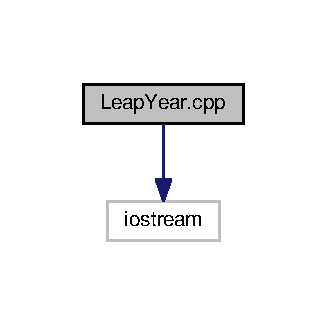
\includegraphics[width=157pt]{LeapYear_8cpp__incl}
\end{center}
\end{figure}
\subsection*{Functions}
\begin{DoxyCompactItemize}
\item 
bool \hyperlink{LeapYear_8cpp_af245d2ce895bb4594869a542fc69e08c}{date\+\_\+checker} (int month, int day, int year)
\item 
bool \hyperlink{LeapYear_8cpp_a999f40dca9542cfd274b59a435946d15}{leap\+\_\+year} (int year)
\item 
void \hyperlink{LeapYear_8cpp_a91b2eb1a7265ee0c01d50c991cac9b1c}{enter\+\_\+date} (int \&month, int \&date, int \&year)
\item 
int \hyperlink{LeapYear_8cpp_ae66f6b31b5ad750f1fe042a706a4e3d4}{main} ()
\end{DoxyCompactItemize}


\subsection{Function Documentation}
\index{Leap\+Year.\+cpp@{Leap\+Year.\+cpp}!date\+\_\+checker@{date\+\_\+checker}}
\index{date\+\_\+checker@{date\+\_\+checker}!Leap\+Year.\+cpp@{Leap\+Year.\+cpp}}
\subsubsection[{\texorpdfstring{date\+\_\+checker(int month, int day, int year)}{date_checker(int month, int day, int year)}}]{\setlength{\rightskip}{0pt plus 5cm}bool date\+\_\+checker (
\begin{DoxyParamCaption}
\item[{int}]{month, }
\item[{int}]{day, }
\item[{int}]{year}
\end{DoxyParamCaption}
)}\hypertarget{LeapYear_8cpp_af245d2ce895bb4594869a542fc69e08c}{}\label{LeapYear_8cpp_af245d2ce895bb4594869a542fc69e08c}

\begin{DoxyCode}
37 \{
38    \textcolor{keywordflow}{switch} (month) \textcolor{comment}{// Checks data in variable month                                                         
                                                                                                       }
39    \{
40       \textcolor{keywordflow}{case} 4:
41       \textcolor{keywordflow}{case} 6:
42       \textcolor{keywordflow}{case} 9:
43       \textcolor{keywordflow}{case} 11:
44          \textcolor{keywordflow}{if} (day >= 1 && day <= 30) \textcolor{comment}{// April, June, Sept., and Nov. have 30 days                           
                                                                                                       }
45             \textcolor{keywordflow}{return} \textcolor{keyword}{true}; \textcolor{comment}{// Returns a true value because the date is valid                                 
                                                                                                       }
46          \textcolor{keywordflow}{else}
47             \textcolor{keywordflow}{return} \textcolor{keyword}{false}; \textcolor{comment}{// Returns a false value because the date is invalid                             
                                                                                                       }
48       \textcolor{keywordflow}{case} 1:
49       \textcolor{keywordflow}{case} 3:
50       \textcolor{keywordflow}{case} 5:
51       \textcolor{keywordflow}{case} 7:
52       \textcolor{keywordflow}{case} 8:
53       \textcolor{keywordflow}{case} 10:
54       \textcolor{keywordflow}{case} 12:
55          \textcolor{keywordflow}{if} (day >= 1 && day <= 31) \textcolor{comment}{// Jan., March, May, July, August, Oct., and Dec. have 31 days         
                                                                                                       }
56             \textcolor{keywordflow}{return} \textcolor{keyword}{true};
57          \textcolor{keywordflow}{else}
58             \textcolor{keywordflow}{return} \textcolor{keyword}{false};
59       \textcolor{keywordflow}{case} 2:
60          \textcolor{keywordflow}{if}(\hyperlink{LeapYear_8cpp_a999f40dca9542cfd274b59a435946d15}{leap\_year}(year)) \textcolor{comment}{// Checks if the year entered is a leap year or not                  
                                                                                                                }
61          \{
62             \textcolor{keywordflow}{if} (day >= 1 && day <= 29) \textcolor{comment}{// February has 29 days during leap years                           
                                                                                                       }
63                \textcolor{keywordflow}{return} \textcolor{keyword}{true};
64             \textcolor{keywordflow}{else}
65                \textcolor{keywordflow}{return} \textcolor{keyword}{false};
66          \}
67          \textcolor{keywordflow}{else}
68          \{
69             \textcolor{keywordflow}{if} (day >= 1 && day <= 28) \textcolor{comment}{// February only has 28 days during years that are not leap years   
                                                                                                       }
70                \textcolor{keywordflow}{return} \textcolor{keyword}{true};
71             \textcolor{keywordflow}{else}
72                \textcolor{keywordflow}{return} \textcolor{keyword}{false};
73          \}
74       \textcolor{keywordflow}{default}: \textcolor{comment}{// The value in month is not 1-12, so there is no corresponding month                       
                                                                                                       }
75          \textcolor{keywordflow}{return} \textcolor{keyword}{false};
76    \}
77 \}
\end{DoxyCode}


Here is the call graph for this function\+:
\nopagebreak
\begin{figure}[H]
\begin{center}
\leavevmode
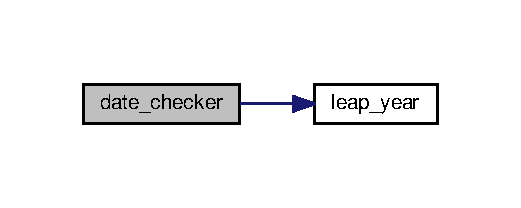
\includegraphics[width=250pt]{LeapYear_8cpp_af245d2ce895bb4594869a542fc69e08c_cgraph}
\end{center}
\end{figure}


\index{Leap\+Year.\+cpp@{Leap\+Year.\+cpp}!enter\+\_\+date@{enter\+\_\+date}}
\index{enter\+\_\+date@{enter\+\_\+date}!Leap\+Year.\+cpp@{Leap\+Year.\+cpp}}
\subsubsection[{\texorpdfstring{enter\+\_\+date(int \&month, int \&date, int \&year)}{enter_date(int &month, int &date, int &year)}}]{\setlength{\rightskip}{0pt plus 5cm}void enter\+\_\+date (
\begin{DoxyParamCaption}
\item[{int \&}]{month, }
\item[{int \&}]{date, }
\item[{int \&}]{year}
\end{DoxyParamCaption}
)}\hypertarget{LeapYear_8cpp_a91b2eb1a7265ee0c01d50c991cac9b1c}{}\label{LeapYear_8cpp_a91b2eb1a7265ee0c01d50c991cac9b1c}

\begin{DoxyCode}
96 \{
97    cout << \textcolor{stringliteral}{"Please enter a date using the following format: mm dd yyyy\(\backslash\)n"};
98    cin >> month >> day >> year; \textcolor{comment}{// The entered data are assigned to the appropriate call-by-reference
       variables                                                                                             }
99 \}
\end{DoxyCode}
\index{Leap\+Year.\+cpp@{Leap\+Year.\+cpp}!leap\+\_\+year@{leap\+\_\+year}}
\index{leap\+\_\+year@{leap\+\_\+year}!Leap\+Year.\+cpp@{Leap\+Year.\+cpp}}
\subsubsection[{\texorpdfstring{leap\+\_\+year(int year)}{leap_year(int year)}}]{\setlength{\rightskip}{0pt plus 5cm}bool leap\+\_\+year (
\begin{DoxyParamCaption}
\item[{int}]{year}
\end{DoxyParamCaption}
)}\hypertarget{LeapYear_8cpp_a999f40dca9542cfd274b59a435946d15}{}\label{LeapYear_8cpp_a999f40dca9542cfd274b59a435946d15}

\begin{DoxyCode}
82 \{
83    \textcolor{keywordflow}{if} (year%400 == 0) \textcolor{comment}{// If a year is divisible by 400, then it is a leap year                             
                                                                                                       }
84       \textcolor{keywordflow}{return} \textcolor{keyword}{true};
85    \textcolor{keywordflow}{else} \textcolor{keywordflow}{if} (year%100 == 0) \textcolor{comment}{// A year that is divisible by 100 but not by 400 is not a leap year            
                                                                                                       }
86       \textcolor{keywordflow}{return} \textcolor{keyword}{false};
87    \textcolor{keywordflow}{else} \textcolor{keywordflow}{if} (year%4 == 0) \textcolor{comment}{// Most years that are divisible by 4 (except the prior examples) are leap years  
                                                                                                       }
88       \textcolor{keywordflow}{return} \textcolor{keyword}{true};
89    \textcolor{keywordflow}{else}
90       \textcolor{keywordflow}{return} \textcolor{keyword}{false};
91 \}
\end{DoxyCode}
\index{Leap\+Year.\+cpp@{Leap\+Year.\+cpp}!main@{main}}
\index{main@{main}!Leap\+Year.\+cpp@{Leap\+Year.\+cpp}}
\subsubsection[{\texorpdfstring{main()}{main()}}]{\setlength{\rightskip}{0pt plus 5cm}int main (
\begin{DoxyParamCaption}
{}
\end{DoxyParamCaption}
)}\hypertarget{LeapYear_8cpp_ae66f6b31b5ad750f1fe042a706a4e3d4}{}\label{LeapYear_8cpp_ae66f6b31b5ad750f1fe042a706a4e3d4}

\begin{DoxyCode}
13 \{
14    \textcolor{keywordtype}{int} month, day, year; \textcolor{comment}{// Variable declarations                                                          
                                                                                                       }
15    \textcolor{keywordtype}{char} ans;
16 
17    cout << \textcolor{stringliteral}{"Welcome to Date Checker!\(\backslash\)n"};
18    cout << endl << \textcolor{stringliteral}{"Now taking inputs from the user ... \(\backslash\)n"};
19    \textcolor{keywordflow}{do}
20    \{
21       \hyperlink{LeapYear_8cpp_a91b2eb1a7265ee0c01d50c991cac9b1c}{enter\_date}(month, day, year); \textcolor{comment}{// Calls function enter\_date                                 
                                                                                                                 }
22 
23       \textcolor{keywordflow}{if}(\hyperlink{LeapYear_8cpp_af245d2ce895bb4594869a542fc69e08c}{date\_checker}(month, day, year)) \textcolor{comment}{// Calls function date\_checker using entered data and
       checks if it returns true                                                                                   
       }
24          cout << \textcolor{stringliteral}{"Date "} << month << \textcolor{stringliteral}{"/"} << day << \textcolor{stringliteral}{"/"} << year << \textcolor{stringliteral}{" is valid.\(\backslash\)n"};
25       \textcolor{keywordflow}{else}
26          cout << \textcolor{stringliteral}{"Date "} << month << \textcolor{stringliteral}{"/"} << day << \textcolor{stringliteral}{"/"} << year << \textcolor{stringliteral}{" is NOT valid.\(\backslash\)n"};
27 
28       cout << \textcolor{stringliteral}{"Do you want to continue? Enter Y or y to continue:\(\backslash\)n"};
29       cin >> ans; \textcolor{comment}{// Assigns entered data into variable ans                                                
                                                                                                       }
30    \} \textcolor{keywordflow}{while} (ans == \textcolor{charliteral}{'y'} || ans == \textcolor{charliteral}{'Y'}); \textcolor{comment}{// If user entered either y or Y, the loop will go again            
                                                                                                       }
31    \textcolor{keywordflow}{return} 0; \textcolor{comment}{// Ends program                                                                               
                                                                                                       }
32 \}
\end{DoxyCode}


Here is the call graph for this function\+:
\nopagebreak
\begin{figure}[H]
\begin{center}
\leavevmode
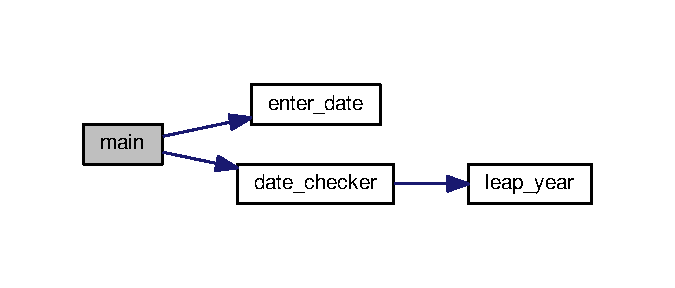
\includegraphics[width=324pt]{LeapYear_8cpp_ae66f6b31b5ad750f1fe042a706a4e3d4_cgraph}
\end{center}
\end{figure}



%--- End generated contents ---

% Index
\backmatter
\newpage
\phantomsection
\clearemptydoublepage
\addcontentsline{toc}{chapter}{Index}
\printindex

\end{document}
